\documentclass[11pt, letterpaper]{article}
\usepackage[left=0.5in, right=0.5in, top=0.5in, bottom=0.75in,]{geometry}
\usepackage{amsthm}
\usepackage{amsmath}
\usepackage{amssymb}
\usepackage{enumitem}
\usepackage{mathtools}
\usepackage{mathrsfs}
\usepackage{fancyhdr}
\usepackage[utf8]{inputenc}
\usepackage{dirtytalk}                      % \say command for quotes
\usepackage{wasysym}
\usepackage{graphicx}
\usepackage{pagecolor}
\usepackage{physics}
\usepackage{tcolorbox}
\tcbuselibrary{skins, breakable}
\usepackage{esint}
\usepackage{subfiles}
\usepackage{hyperref}
\usepackage{graphicx}
\usepackage{listings}
\usepackage{subfig}
\usepackage{caption}
\usepackage{xcolor}
\usepackage{tikz}
\hypersetup{                                % Formatting for hyperlinks
    colorlinks,
    citecolor=black,
    filecolor=black,
    linkcolor=black,
    urlcolor=black
}

\title{\vspace{-1cm}\bf Competitive Programming Algorithms}
\author{}
\date{}

\definecolor{codegreen}{rgb}{0,0.6,0}
\definecolor{codegray}{rgb}{0.5,0.5,0.5}
\definecolor{codepurple}{rgb}{0.58,0,0.82}
\definecolor{backcolour}{rgb}{0.95,0.95,0.92}

\lstdefinestyle{mystyle}{
    language=C++,
    backgroundcolor=\color{backcolour},
    commentstyle=\color{codegreen},
    keywordstyle=\color{magenta},
    numberstyle=\tiny\color{codegray},
    stringstyle=\color{codepurple},
    basicstyle=\ttfamily\footnotesize,
    breakatwhitespace=false,
    breaklines=true,
    captionpos=b,
    keepspaces=true,
    numbers=left,
    numbersep=5pt,
    showspaces=false,
    showstringspaces=false,
    showtabs=false,
    tabsize=4,
    frame=lines,
}
\lstset{style=mystyle}

\setlength{\parindent}{0pt}
\begin{document}

\maketitle
\tableofcontents
\pagebreak

% Introduction and Miscellaneous
\section{Introduction and Miscellaneous}

\begin{center}
    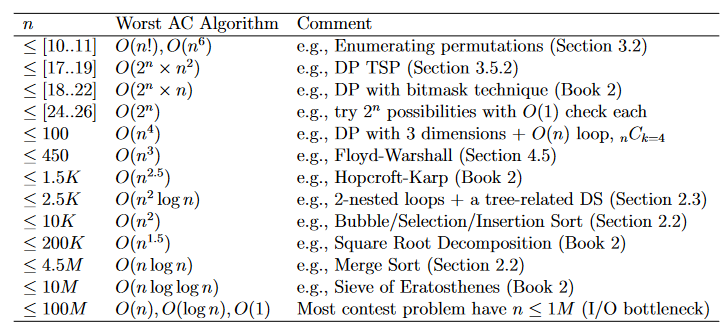
\includegraphics[scale=0.65]{assets/table.png}
\end{center}

\subsection{Template}
\lstinputlisting{code/miscellaneous/template.cpp}

\subsection{Codeforces Template}
\lstinputlisting{code/miscellaneous/codeforces_template.cpp}

\subsection{Generate Files}
\lstinputlisting[language=Bash]{code/miscellaneous/generate_files.sh}

\subsection{Binary Search}
\lstinputlisting{code/miscellaneous/binary_search.cpp}

\subsection{Base 10 to Base $m$}
\lstinputlisting{code/miscellaneous/base_10_to_base_m.cpp}

\subsection{Coordinate Compression}
\lstinputlisting{code/miscellaneous/coordinate_compression.cpp}

% Data Structures
\section{Data Structures}

\subsection{Order Statistic Tree (Set)}
\lstinputlisting{code/data_structures/order_statistic_tree_(Set).cpp}

\subsection{Order Statistic Tree (Map)}
\lstinputlisting{code/data_structures/order_statistic_tree_(Map).cpp}

\subsection{Union Find}
\lstinputlisting{code/data_structures/union_find.cpp}

\subsection{Sparse Table}
\lstinputlisting{code/data_structures/sparse_table.cpp}

\subsection{Range Tree}
\lstinputlisting{code/data_structures/range_tree.cpp}

\subsection{Range Tree on Trees}
\lstinputlisting{code/data_structures/range_tree_on_trees.cpp}

% Dynamic Programming
\section{Dynamic Programming}

\subsection{Knapsack}
\lstinputlisting{code/dynamic_programming/knapsack.cpp}

\subsection{Bitsets}
\lstinputlisting{code/dynamic_programming/bitsets.cpp}

\subsection{Travelling Sales Person}
\lstinputlisting{code/dynamic_programming/travelling_sales_person.cpp}

% Graph Algorithms
\section{Graph Algorithms}

\subsection{Breath First Search}
\lstinputlisting{code/graph_algorithms/breath_first_search.cpp}

\subsection{Depth First Search}
\lstinputlisting{code/graph_algorithms/depth_first_search.cpp}

\subsection{Bridge Finding}
\lstinputlisting{code/graph_algorithms/bridge_finding.cpp}

\subsection{Directed Cycle Detection}
\lstinputlisting{code/graph_algorithms/directed_cycle_detection.cpp}

\subsection{Tree Representation}
\lstinputlisting{code/graph_algorithms/tree_representation.cpp}

\subsection{Binary Lifting}
\lstinputlisting{code/graph_algorithms/binary_lifting.cpp}

\subsection{Kosaraju's Algorithm}
\lstinputlisting{code/graph_algorithms/kosaraju's_algorithm.cpp}

\subsection{Topological Sort}
\lstinputlisting{code/graph_algorithms/topological_sort.cpp}

\subsection{Compute SCC DAG}
\lstinputlisting{code/graph_algorithms/compute_SCC_DAG.cpp}

\subsection{2-SAT}
\lstinputlisting{code/graph_algorithms/(Two)_2-SAT.cpp}

\subsection{Kruskal's Algorithm}
\lstinputlisting{code/graph_algorithms/kruskal's_algorithm.cpp}

\subsection{Prim's Algorithm}
\lstinputlisting{code/graph_algorithms/prim's_algorithm.cpp}

\subsection{Shortest Path Algorithms}
\subsubsection{Dijkstra's Algorithm}
\lstinputlisting{code/graph_algorithms/shortest_path_algorithms/dijkstra's_algorithm.cpp}

\subsubsection{Bellman Ford}
\lstinputlisting{code/graph_algorithms/shortest_path_algorithms/bellman_ford.cpp}

\subsubsection{Finding Negative Cycles}
\lstinputlisting{code/graph_algorithms/shortest_path_algorithms/finding_negative_cycles.cpp}

\subsubsection{Floyd Warshall}
\lstinputlisting{code/graph_algorithms/shortest_path_algorithms/floyd_warshall.cpp}

% Flow Networks
\section{Flow Networks}

\subsection{Dinic's Algorithm}
\lstinputlisting{code/flow_networks/dinic's_algorithm.cpp}

\subsection{Min-cut}
\lstinputlisting{code/flow_networks/min-cut.cpp}

% Mathematics
\section{Mathematics}

\subsection{Fast Exponentiation}
\lstinputlisting{code/mathematics/fast_exponentiation.cpp}

\subsection{Primality Testing}
\lstinputlisting{code/mathematics/primality_testing.cpp}

\subsection{Prime Factorisation}
\lstinputlisting{code/mathematics/prime_factorization.cpp}

\subsection{Sieve of Eratosthenes}
\lstinputlisting{code/mathematics/sieve_of_eratosthenes.cpp}

\subsection{GCD}
\lstinputlisting{code/mathematics/GCD.cpp}

\subsection{LCM}
\lstinputlisting{code/mathematics/LCM.cpp}

\subsection{Extended Euclidean Algorithm}
\lstinputlisting{code/mathematics/extended_euclidean_algorithm.cpp}

\subsection{Matrices}
\lstinputlisting{code/mathematics/matrices.cpp}

\subsection{Combinations}
\lstinputlisting{code/mathematics/combinations.cpp}

% Computational Geometry
\section{Computational Geometry}

\subsection{Cross Product}
\lstinputlisting{code/computational_geometry/cross_product.cpp}

\subsection{Three Points Collinear}
\lstinputlisting{code/computational_geometry/three_points_collinear.cpp}

\subsection{Segment-Segment Intersection}
\lstinputlisting{code/computational_geometry/segment-segment_intersection.cpp}

\subsection{Polygon Area (Trapezoidal Rule)}
\lstinputlisting{code/computational_geometry/polygon_area_(Trapezoidal Rule).cpp}

\subsection{Polygon Area (Cross Product)}
\lstinputlisting{code/computational_geometry/polygon_area_(Cross Product).cpp}

\subsection{Convex Hull}
\lstinputlisting{code/computational_geometry/convex_hull.cpp}

\subsection{Half Plane Intersection}
\lstinputlisting{code/computational_geometry/half_plane_intersection.cpp}

\end{document}
